\documentclass[research]{BMSTU-IU8}

\usepackage{
    listingsutf8,
    pdfpages,
    tikz,
    pgf-umlcd,
    mathtools,
    braket,
    % Ажурные символы.
    amsfonts
}
\usetikzlibrary{trees,positioning}

\student{А.Н. Александров}
\theme{Разработка средства обнаружения аномалий сетевых пакетов на основе машинного обучения}
\group{ИУ8-124}
\supervisor{Н.С. Коннова}
\studentFullName{Александров Алексей Николаевич}
\profile{19У113}
\speciality{10.05.01 <<Компьютерная безопасность>>}
\specialization{10.05.01\_01 <<Математические методы защиты информации>>}
\supervisorWithDegree{к.т.н., доцент кафедры ИУ8, Коннова Н.С.}

% redundant, yet required variable definitions
\researchConsultant{}
\designConsultant{}
\technologicalConsultant{}
\economicsConsultant{}
\lawsConsultant{}
\normController{}

\addbibresource{main.bib}

\usepackage{}

\defbibenvironment{nirs-bibliography}
  {\list
     {\printfield{labelnumber}}
     {\setlength{\leftmargin}{0pt} % устанавливаем отступ слева
      \setlength{\itemindent}{4.0em} % устанавливаем отступ для номера
      \setlength{\parsep}{\parskip}}
     \renewcommand*{\makelabel}[1]{\hss##1}}
  {\endlist}
  {\item}

\makeatletter
% +10mm ко всем сдвигам
\renewcommand*\l@section{\@dottedtocline{0}{10mm}{2em}}
\renewcommand*\l@structure{\@dottedtocline{0}{10mm}{0em}}
\renewcommand*\l@subsection{\@dottedtocline{1}{15mm}{3em}}
\renewcommand*\l@subsubsection{\@dottedtocline{2}{20mm}{4em}}
\renewcommand*\l@paragraph{\@dottedtocline{3}{25mm}{5em}}
\makeatother

\begin{document}
    \IfFileExists{inc/titul.pdf}
    {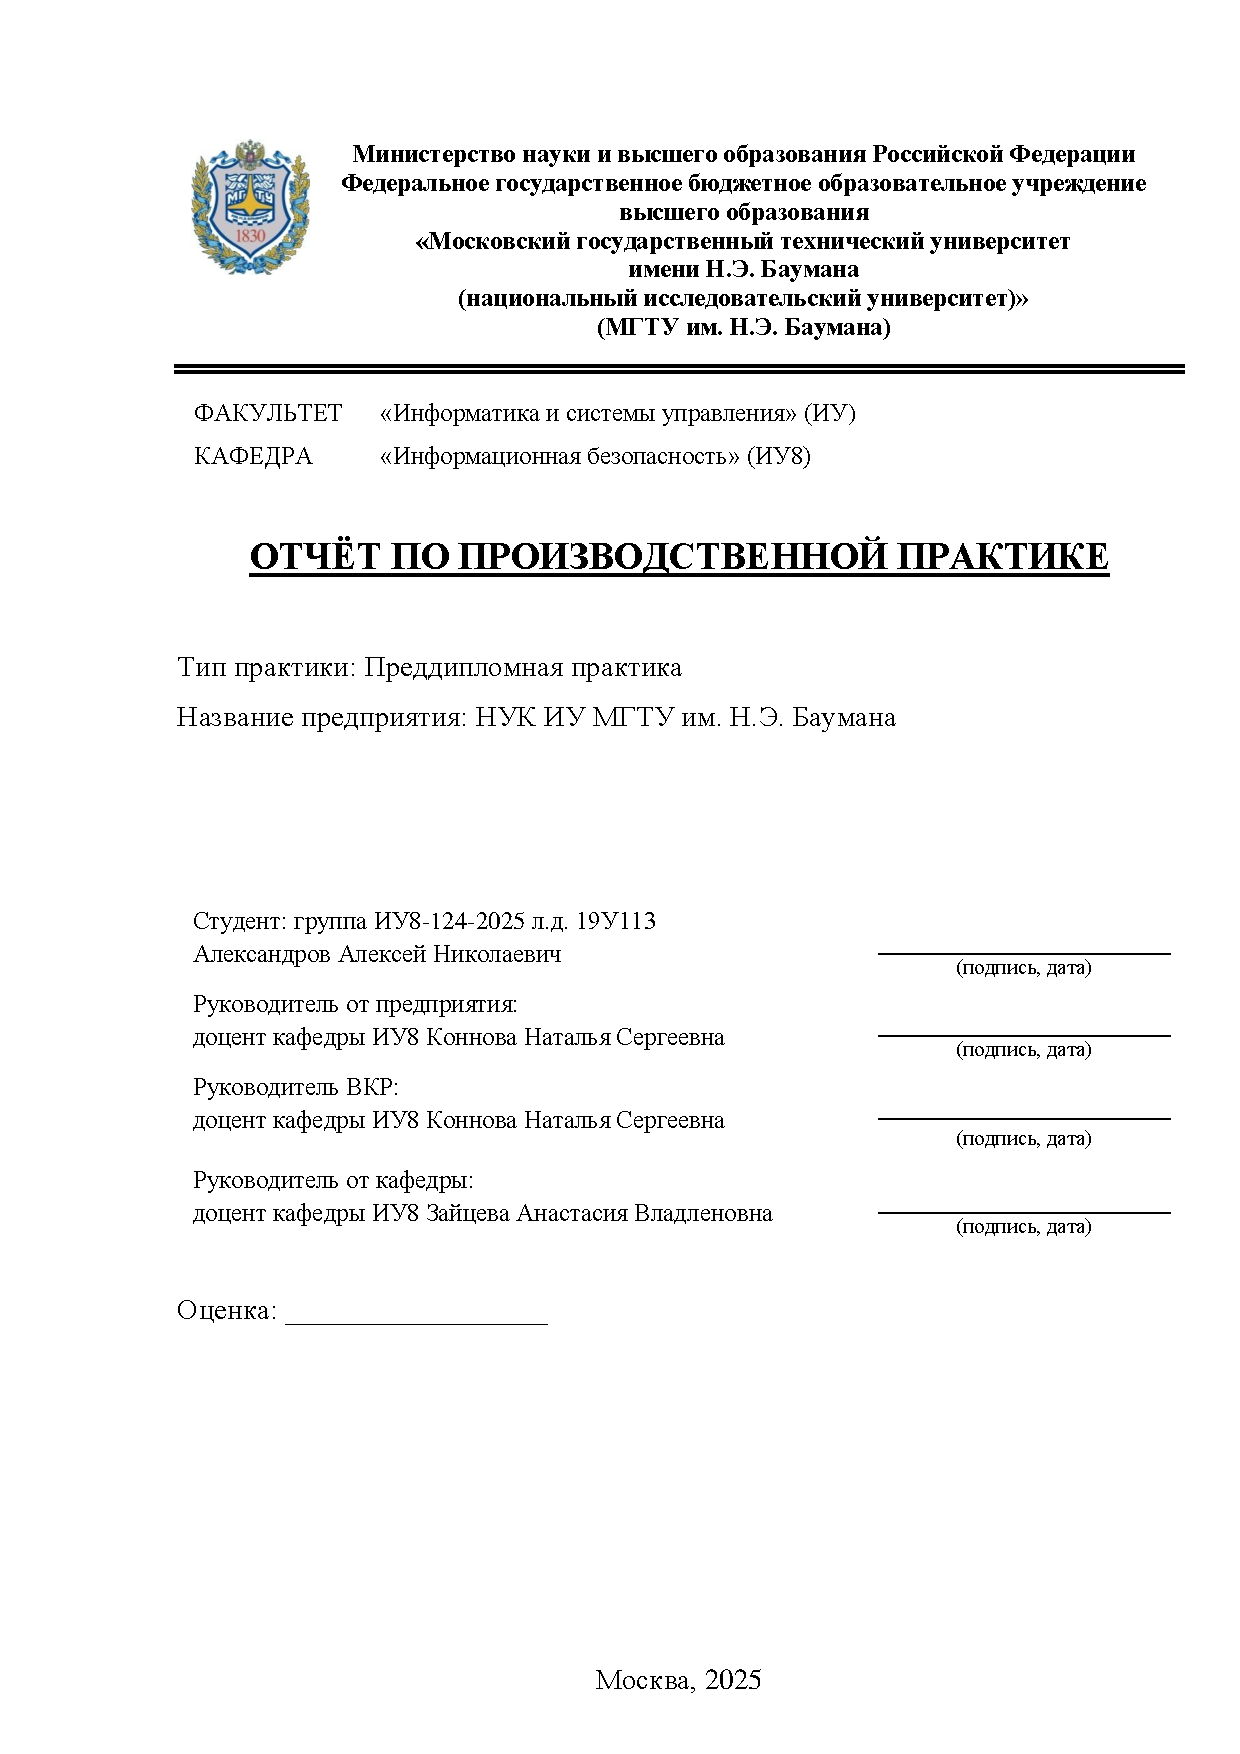
\includepdf[pages=-]{inc/titul}}
    {\maketitle}
    \setcounter{page}{3}

    \tableofcontents

    \introduction

В современном информационном обществе огромное количество данных поступает из различных источников, таких как сети передачи данных, датчики, мобильные устройства и облачные платформы. Обработка и анализ этих данных стали неотъемлемой частью многих сфер, однако одним из серьезных вызовов является обнаружение аномалий в данных, которые могут свидетельствовать о наличии угроз безопасности или нештатных ситуациях. В этом контексте, проблема обнаружения аномалий в данных выходит на первый план. Аномалии могут служить индикаторами возможных атак, ошибок в данных или других проблем, которые могут существенно повлиять на надежность и безопасность информационных систем.

Под аномалией или выбросом (от англ. outlier) \cite{What-is-anomalies} понимают любой несогласованный или избыточный экземпляр выборки, отличающийся от базовой модели. Обычно это происходит, когда данные отклоняются от установленного набора данных по различным причинам, например, при неполной загрузке или неожиданном удалении информации в базе данных. Обнаружение аномалий помогает отладить процесс выявления выбросов и их устранения во избежание дефектов в наборе данных.
В условиях постоянного роста объема данных, методы машинного обучения \cite{Outliers-in-data} обеспечивают эффективную обработку больших массивов информации. Также важным преимуществом является способность выявлять сложные и неочевидные закономерности в данных, что делает их более эффективными в обнаружении аномалий.

С появлением больших данных и широкого использования информационных технологий возросла необходимость в создании эффективных \cite{AI-and-ML-for-AD} средств обнаружения аномалий в данных. В зависимости от предметной области и конкретной информационной системы, аномалии могут быть признаком несанкционированного доступа, вредоносной активности или технических сбоев.

В целом, некорректные данные могут привести к неправильным аналитическим выводам, неправильным рекомендациям и даже серьезным финансовым и организационным потерям. Так недавнее исследование SAS (американская компания-разработчик систем класса Busyness Intelligence и ПО для статистического анализа) \cite{SAS-Data-Quality} в Европе показало растущую важность качества данных в финансовой сфере. 66\% европейских компаний подтвердили, что ошибки в данных негативно влияют на прибыль, 74\% процента из них приняли меры по решению проблем качества данных. В связи с этим возникает потребность в совершенствовании методов анализа данных, способных оперативно выявлять нештатные ситуации.

В частности, обнаружение аномалий методами машинного обучения имеет широкий спектр применения и приложений: обнаружение инцидентов информационной безопасности по аномалиям \cite{Method-detection-incidents-IS}, выявление неисправностей в технических системах и IoT \cite{Diagnostics-IoT}, выявление мошеннической деятельности и фальсификаций \cite{Detection-anomalies-and-falsifications}. Выбор методов на основе ML также связан с способностью обнаружения неявных и сложных закономерностей в данных \cite{ML-powered-AD}, что обеспечивает эффективное выявление аномалий, которые могли бы быть упущены традиционными методами. Возможность обучаться на основе больших объемов данных, является эффективной в обнаружении новых, ранее неизвестных типов аномалий.

Место прохождения практики – Научно-учебный комплекс «Информатика и системы управления» МГТУ им. Н.Э. Баумана. Период прохождения практики – с 7 февраля 2025 г. по 7 марта 2025 г.

Цели прохождения практики – сформулировать и предложить варианты решения математической постановки задачи обнаружения аномалий в сетевом трафике на основе машинного обучения.

Задачи прохождения практики:

\begin{itemize}[leftmargin=0pt,itemindent=4.6em]
    \item[$\bullet$] Предложить формулировку математической постановки задачи обнаружения аномалий в сетевом трафике на основе машинного обучения.

    \item[$\bullet$] Рассмотреть, проанализировать и предложить возможные пути решения поставленной задачи.

    \item[$\bullet$] Представить выбор и обоснование решения математической постановки настоящей задачи.
\end{itemize}

    \structure{ОСНОВНАЯ ЧАСТЬ}

В рамках прохождения преддипломной практики был подготовлен настоящий отчёт о проделанной работе. Основная часть состоит из четырёх основных разделов, затрагивающих формулировку и решение математической постановки задачи обнаружения аномалий в сетевом трафике на основе машинного обучения.

Основными объектами изучения стали актуальные подходы к детектированию аномалий сетевых пакетов, выбор оптимального алгоритма решения данной проблемы, а также математический аппарат, используемый применительно к формализации и описанию рассматриваемой задачи.

В первом разделе представлена характеристика организации Научно-учебного комплекса «Информатика и системы управления» (НУК ИУ) МГТУ им. Н.Э. Баумана, где описаны цели и задачи данного подразделения, а также его роль в образовательном и научном процессах.

Во втором разделе формулируется математическая постановка задачи, где вводится множество экземпляров сетевой активности и их признаковое описание. Определяются метки классов для аномальных и нормальных экземпляров, а также формулируется функция принятия решений, позволяющая классифицировать данные. Также рассматриваются ошибки I-го и II-го рода, их взаимосвязь, позволяющую выйти на окончательную формулировку задачи. 

Следующий, третий раздел посвящён обзору и описанию различных методов и подходов к решению сформулированной задачи. В этом разделе производится анализ существующих методов, таких как критерий <<трёх сигм>>, одноклассовый метод опорных векторов, изолирующий лес и автокодировщики. В заключение, сделан выбор в пользу одного из методов, обоснованный его эффективностью и соответствием требованиям задачи. Это позволит не только продемонстрировать практическую значимость проведённой работы, но и предложить рекомендации по дальнейшему развитию и улучшению систем обнаружения аномалий в сетевом трафике.

    \section{Характеристика организации}

Научно-учебный комплекс «Информатика и системы управления» \cite{Requlations-SEC-ISC} (далее --- НУК ИУ) является самостоятельным структурным подразделением МГТУ им. Н.Э. Баумана (далее --- Университет). Полное наименование НУК ИУ на английском языке Scientific Educational Complex «Informatics and Control Systems» Bauman Moscow State Technical University. Сокращённое --- SEC ICS BMSTU.

НУК ИУ возглавляет руководитель НУК ИУ д.т.н., профессор и заведующий кафедрой ИУ6 («Компьютерные системы и сети») Пролетарский А.В., который непосредственно подчиняется действующему ректору Университета к.т.н. Гордину М.В..

Цель деятельности НУК ИУ: обеспечение образовательного и научного процессов в соответствии с Уставом Университета. К основным задачам подразделения относят:

\begin{itemize}[leftmargin=0pt,itemindent=4.6em]
    \item Подготовку бакалавров, специалистов, магистров, научных и научно-педагогических кадров высшей квалификации в соответствии с государственными лицензиями, выданными Университету. 
        
    \item Выполнение фундаментальных, поисковых и прикладных научных исследований, проведение опытно-конструкторских работ и производство опытных образцов перспективной техники и технологий. 
        
    \item Написание и издание учебников, учебных пособий и монографий. 
        
    \item Развитие научных, педагогических и инженерных школ НУК ИУ. 

    \item Разработку и внедрение прогрессивных форм, методов и средств подготовки специалистов. 

    \item Повышение квалификации и переподготовка научно-педагогических кадров технических и экономических учебных заведений, а также специалистов предприятий с высшим образованием. 

    \item Развитие материально-технической базы НУК ИУ. 

    \item Организацию научной работы студентов. 

    \item Развитие различных форм сотрудничества с высшими учебными заведениями России и зарубежных стран. 

    \item Социальную поддержку и защиту преподавателей, научного и отвечающих требованиям подготовки вспомогательного персонала. 
\end{itemize}


    \section{Математическая постановка задачи}

Пусть $T = \{t_1, t_2, \ldots , t_k\}$ --- множество экземпляров сетевой активности. Каждому из объектов данного множества по формуле (\ref{X_def}) поставим в соответствие \textit{признаковое описание}, полученное биекцией $\xi: T \rightarrow X, \ |T| = |X| = k$.

\begin{equation}\label{X_def}
    X = \{\overline{x_i} = \xi(t_i)\ |\ \forall t_i \in T\} = \{\overline{x_1}, \overline{x_2}, \ldots , \overline{x_k}\},
\end{equation}
где каждый вектор $\overline{x_i},\ i = \overline{1,k}$ представляет собой набор характеристик, которые достаточно полно описывают соответствующий экземпляр $t_i$ в рамках данной задачи.

Также соотношением (\ref{Y_def}) определим множество меток классов принадлежности экземпляров из $T$ к аномальному трафику:
\begin{equation}\label{Y_def}
    Y = \{y_1,\ y_2\},
\end{equation}
где    $y_1$ --- метка класса аномальных экземпляров (или <<аномальные>>); \\
$y_2$ --- метка класса экземпляров без аномалий (или <<нормальные>>).

По формуле (\ref{f_def}) кусочно зададим функцию принятия решений $f$, которая для каждого экземпляра $t_i \in T$ на основе соответствующего вектора признаков $\overline{x_i} \in X$, однозначно позволяет определить метку класса из $Y$:

\begin{equation}\label{f_def}
    f(\overline{x_i}) = \begin{cases}
            \ \ 1, &\ \text{если } \overline{x_i} \text{ соответствует классу }y_1, \\
               -1, &\ \text{если } \overline{x_i} \text{ соответствует классу }y_2, \\ 
         \end{cases}
\end{equation}
где оценку корректности функции $f$ можно получить с помощью ошибок первого и второго рода.

Ошибкой I-го рода ($\alpha$-ошибкой, ложноположительным заключением, англ. false positive) будем называть ситуацию, при которой функция $f$ отнесёт экземпляр $t_i \in T$ к классу $y_1$ (<<аномальных>>), хотя фактически он является <<нормальным>>, то есть относится к классу $y_2$. Вероятность возникновения данного типа ошибки (также называемая \textit{уровнем значимости}) определяется соотношением (\ref{alpha_def}).

\begin{equation}\label{alpha_def}
    \alpha = P \Big\{ f(\overline{x_i}) = 1 \ \Big|\ t_i\ -\ \text{«нормальный» экземпляр} \Big\}
\end{equation}

Ошибкой II-го рода ($\beta$-ошибкой, ложноотрицательное заключением, англ. false negative) будем называть ситуацию, при которой функция $f$ отнесёт экземпляр $t_i \in T$ к классу $y_2$ (<<нормальных>>), хотя фактически он является <<аномальным>>, то есть относится к классу $y_1$. Вероятность возникновения данного типа ошибки по аналогии определяется соотношением (\ref{beta_def}).

\begin{equation}\label{beta_def}
    \beta = P \Big\{ f(\overline{x_i}) = -1 \ \Big|\ t_i\ -\ \text{«аномальный» экземпляр} \Big\}
\end{equation}
Также с этой величиной тесно связана другая, имеющая большое статистическое значение --- \textit{мощность критерия} $(1 - \beta)$. Таким образом, чем выше мощность критерия, тем меньше вероятность совершить ошибку второго рода.

Ошибки первого и второго рода взаимосвязаны между собой: при снижении уровня значимости увеличивается вероятность пропуска аномального трафика (уменьшается мощность критерия). В контексте текущей задачи, ошибка II-го рода может иметь более серьезные последствия, так как пропуск аномального трафика может привести к утечке данных или другим угрозам безопасности. В то же время, распространение ошибки I-го рода может негативно сказаться на пользовательском опыте администраторов и операторов разрабатываемой системы, поскольку это приводит к избыточной обработке и разбору ложноположительных инцидентов.

В результате задача, представленная в (\ref{task_formulation}),  заключается в минимизации вероятности ошибки второго рода при классификации, при этом на уровень значимости $\alpha$ накладывается ограничение значением порога $p$, которое определяет допустимый уровень ошибки I-го рода:

\begin{equation}\label{task_formulation}
    \begin{cases}
         \beta \rightarrow \min\limits_{
            \substack{
                \overline{x_i}\ :=\ \xi(t_i) \\
                f(\overline{x_i})
            }
        },
        \\
        \alpha \leq p.
    \end{cases}
\end{equation}

На основании исследований, представленных в работах \cite{Threshold-Adaptation}, \cite{Vasilyev-IS}, \cite{Detect-Anomalies-Deep-NN} принято решение установить пороговое значение ошибки первого рода на уровне $p = 0,05$, что позволит обеспечить баланс между безопасностью и удобством использования системы. Это значение будет использоваться для настройки алгоритмов классификации и оптимизации их работы. Также оно будет проверено результатами проводимых численных экспериментов.



    \section{Пути решения поставленной задачи}

В данном разделе представлены некоторые методы и подходы к решению сформулированной выше задачи. 

Первый подход, который будет рассмотрен, это классический статистический метод -- критерий <<трёх сигм>>, основанный на предположении о нормальном распределении данных и позволяет выявлять аномалии, находящиеся за пределами трех стандартных отклонений от среднего значения. Несмотря на свою простоту и легкость в реализации, данный метод имеет ограничения, особенно в случаях, когда данные не подчиняются нормальному распределению.

Следующим методом является одноклассовый метод опорных векторов (One-Class SVM). Этот подход позволяет выделять области с высокой плотностью данных и эффективно обнаруживать аномалии, используя концепцию гиперплоскостей в пространстве признаков. One-Class SVM демонстрирует высокую эффективность в задачах, где аномальные данные редки и сложно выделяются.

Третий метод, который будет обсужден, это изолирующий лес (Isolation Forest). Этот алгоритм основан на принципе, что аномалии легче изолировать, так как они редки. Изолирующий лес использует случайные деревья для разделения данных и позволяет быстро и эффективно обнаруживать аномалии в больших объемах данных. В дополнение к этому, будет рассмотрено расширение данного метода — Deep Isolation Forest, которое улучшает результаты за счет использования нейронных сетей.

Также будет представлен алгоритм ECOD (Empirical-Cumulative-distribution-based Outlier Detection), который использует эмпирическую кумулятивную функцию распределения для оценки вероятности появления аномалий. Этот метод отличается простотой и отсутствием гиперпараметров, что делает его удобным для практического применения.

Наконец, в разделе будет рассмотрено применение автокодировщиков для обнаружения аномалий. Автокодировщики представляют собой нейронные сети, которые обучаются восстанавливать нормальные данные и могут быть использованы для выявления аномалий на основе ошибки восстановления. Этот подход позволяет эффективно обрабатывать сложные данные и выявлять аномалии, которые не были представлены в обучающем наборе.
    \subsection{Критерий <<трёх сигм>>}

Для начала рассмотрим классический и основополагающий метод обнаружения аномалий с использованием критерия <<трех сигм>>. Этот метод является статистическим и основывается на предположении, что данные распределены нормально, и аномалии могут быть выявлены как те, которые выходят за пределы трех среднеквадратичных отклонений от среднего значения.

Из простоты метода следуют очевидные ограничения на область его применения: при значительном отклонении данных от распределения Гаусса эффективность и точность метода может значительно снизиться.

Для использования критерия необходимо рассчитать среднее значение и стандартное отклонение по формулам (\ref{average}) и (\ref{standard_deviation}) соответственно.

\begin{equation}\label{average}
    \mu = \frac{1}{n} \sum\limits_{i = 1}^{n}x_i,
\end{equation}

\begin{equation}\label{standard_deviation}
    \sigma = \sqrt{\frac{1}{n} \sum\limits_{i = 1}^{n}(x_i - \mu)^2},
\end{equation}
где $n$ – количество элементов выборки, $x_i$ --- $i$-ый элемент выборки.

Затем аномалии определяются как те значения, которые находятся за пределами интервала, определенного трех среднеквадратичных отклонений от среднего (см. рисунок~\ref{fig:three-sigma}).

\begin{figure}
  \centering
  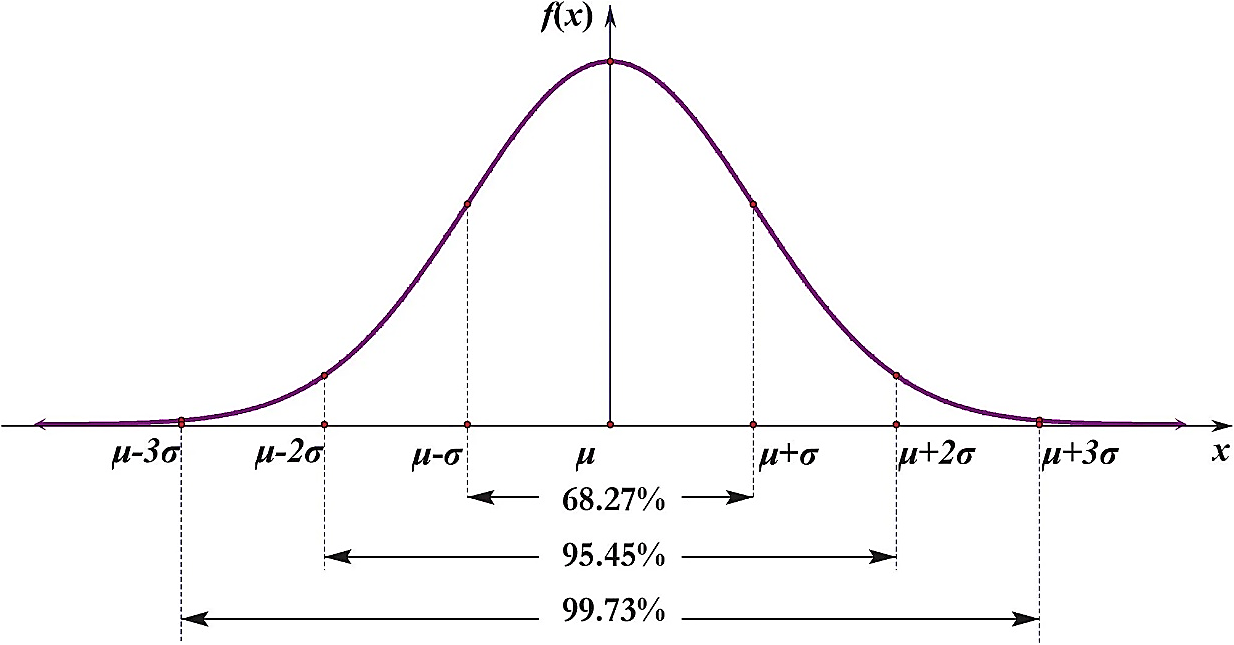
\includegraphics[scale=0.3]{inc/images/three-sigma.png}
  \caption{График нормального распределения и процент попадания в отрезки, равные среднеквадратичному отклонению \cite{Three-Sigma-Limits}}
  \label{fig:three-sigma}
\end{figure}

Помимо своей простоты, данный метод имеет ограничения в эффективности при обнаружении сложных нелинейных закономерностей в данных. Кроме того, такой подход не учитывает структуру данных и контекст анализа. Однако он включён рассмотрение ввиду его первоначальной каноничности для решения поставленной задачи. Многие статистические модели используют, развивают и усовершенствуют данный подход.

При использовании критерия <<трёх сигм>> формулируется функция принятия решения, которая непосредственно соответствует постановке задачи. В частности, определяем функцию (\ref{f_3sigma}):
\begin{equation}\label{f_3sigma}
    f(\overline{x_i}) = \begin{cases}
         \ \ 1, & \text{если } |\overline{x_i} - \mu| > 3\sigma, \\
        -1, & \text{если } |\overline{x_i} - \mu| \le 3\sigma,
    \end{cases}
\end{equation}
где $\mu$ и $\sigma$ вычисляются по формулам (\ref{average}) и (\ref{standard_deviation}). Таким образом, наблюдение $\overline{x_i}$ классифицируется как аномальное (метка $y_1$) при условии, что его отклонение от среднего превышает три стандартных отклонения.

\textit{При нормальном распределении признаков} вероятность ложноположительного срабатывания определяется выражением (\ref{alpha_3sigma}), а вероятность ошибки II-го рода --- соотношением (\ref{beta_3sigma}).
\begin{equation}\label{alpha_3sigma}
    \alpha = P\Big\{ |\overline{x_i} - \mu| > 3\sigma\ \Big|\ t_i\ -\ \text{«нормальный» экземпляр} \Big\},
\end{equation}

\begin{equation}\label{beta_3sigma}
    \beta = P\Big\{ |\overline{x_i} - \mu| \le 3\sigma\ \Big|\ t_i\ -\ \text{«аномальный» экземпляр} \Big\}.
\end{equation}
что удовлетворяет установленному ограничению $\alpha \leq p$, где порог $p$ выбран равным 0,05.

Таким образом метод, позволяет установить строгие границы для функции принятия решения $f$. При условии нормальности распределения данных, критерий <<трёх сигм>> обеспечивает очень малую вероятность ошибки I-го рода, что удовлетворяет ограничению, заданному в постановке задачи, и позволяет эффективно минимизировать $\beta$, что соответствует цели оптимизации, сформулированной в (\ref{task_formulation}). Однако сетевой трафик редко может быть описан распределением Гаусса, ввиду нерегулярности событий в вычислительных сетях, что даёт повод для рассмотрения других путей решения задачи.

    \subsection{Одноклассовый метод опорных векторов, One-Class SVM}

One-Class Support Vector Machine (One-Class SVM или просто One-SVM) представляет собой одноклассовый неконтролируемый метод обнаружения аномалий \cite{Skilear-One-Class-SVM-Doc}. Основной идеей One-SVM является установление границы, охватывающей области с высокой плотностью данных, при этом исключая заданную долю данных $\nu = (0;\ 1]$ (гиперпараметр модели), которая (по мнению пользователя модели) представляет собой верхнюю границу числа аномалий в данных (см. рисунок \ref{fig:one-class-svm}).

\begin{figure}
  \centering
  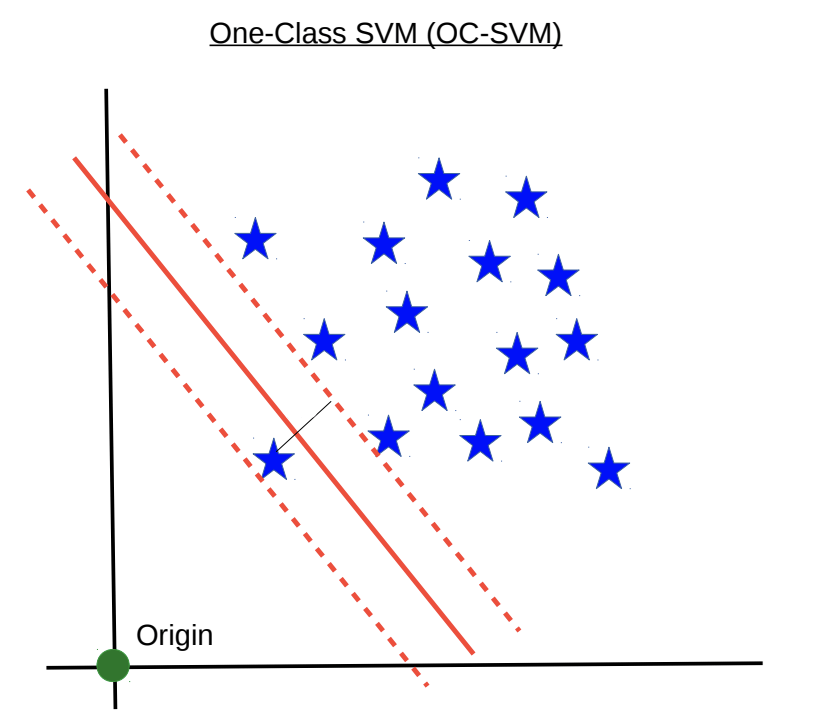
\includegraphics[scale=0.5]{inc/images/one-class-svm.png}
  \caption{Специализация метода опорных векторов для поиска выбросов \cite{SVM-Lecture}}
  \label{fig:one-class-svm}
\end{figure}

Главной целью One-SVM является поиск гиперплоскости, разделяющей данные от источника (начала координат). Для достижения этой цели метод использует линейный классификатор, но с использованием ядра --- функции, которая отображает пространство признаков в пространство высшей размерности. Канонично данный kernel trick \cite{Anomaly-Detection-One-Class-SVM} позволяет разделять классы, линейно неразделимые в текущем признаковом пространстве (см. рисунок \ref{fig:nonlinear-separation-demo}). Таким образом на выходе получается модель с нелинейными границами в исходном пространстве переменных задачи.

\newpage

RBF (Radial Basis Function) \cite{RBF-Kernel-in-SVM} часто является наиболее широко применяемым ядром для One-SVM ввиду нелинейности и гибкой адаптации к различным распределениям данных. Данное ядро определяется функцией (\ref{RBF_def}):

\begin{equation}\label{RBF_def}
    K_{RBF}(\overline{x},\ \overline{x}') = e^{-\gamma \lVert \overline{x} - \overline{x}' \rVert^2},
\end{equation}
где $\overline{x},\ \overline{x}' \in \mathbb{R}^k$ --- выборки, векторы в входном пространстве размерности $k$, \\
$\gamma$ --- свободный параметр, который позволяет настраивать влияние соседних точек на границу принятия решения.

\begin{figure}
  \centering
  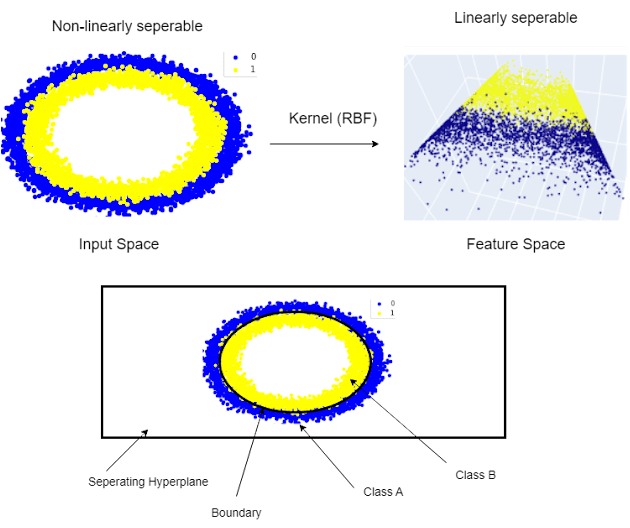
\includegraphics[scale=0.45]{inc/images/nonlinear-separation-demo.png}
  \caption{Нелинейное разделение данных на основе пороговой гиперплоскости в пространстве признаков \cite{RBF-Kernel-in-SVM}}
  \label{fig:nonlinear-separation-demo}
\end{figure}

Таким образом, в результате обучения One-Class SVM стремится создать гиперплоскость, которая наилучшим образом ограничит область с высокой плотностью данных (см. рисунок \ref{fig:rbf-demo}), считая все остальные области аномальными. Этот метод демонстрирует свою эффективность в выявлении аномалий и обеспечивает контроль над тем, какая доля данных считается аномальной, благодаря гиперпараметру $\nu$.

\begin{figure}
  \centering
  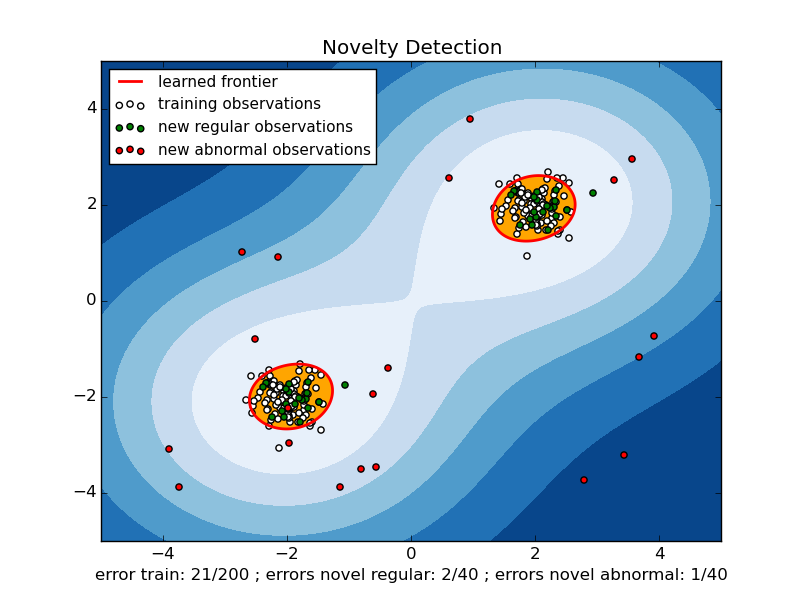
\includegraphics[scale=0.3]{inc/images/rbf-demo.png}
  \caption{Пример обнаружения аномалий на основе One-SVM с нелинейным ядром RBF \cite{Skilear-RBF-Doc}}
  \label{fig:rbf-demo}
\end{figure}

% При использовании One-Class SVM функция принятия решения решений можно формализовать соотношением (\ref{f_ocsvm}).
% \begin{equation}\label{f_ocsvm}
%     f(\overline{x_i}) = sign\Big[K(\overline{x_i},\ \overline{x_j}) - b\Big],
% \end{equation}
% где $K$ --- функция ядра (может быть определена, как в формуле (\ref{RBF_def})), \\
% $\overline{w}$ --- весовые коэффициенты, корректирующиеся в процессе обучения модели, \\
% $b$ --- пороговое значение смещения, которое задаёт сдвиг гиперплоскости относительно начала координат.

% Ключевой гиперпараметр $\nu \in (0,\ 1]$ задаёт максимальную допустимую долю аномальных экземпляров в данных, что позволяет установить ограничение на вероятность ложноположительного срабатывания:
% \begin{equation}\label{alpha_ocsvm}
%     \alpha = P\Big\{ f(\overline{x_i}) = 1\ \Big|\ t_i\ -\ \text{«нормальный» экземпляр} \Big\} \leq p,
% \end{equation}
% где, при корректном выборе $\nu$, порог $p$ (например, $0,05$) выполняется.

% При этом модель стремится инкапсулировать область с высокой плотностью нормальных данных, минимизируя вероятность ошибки II-го рода, которая определяется как
% \begin{equation}\label{beta_ocsvm}
%     \beta = P\Big\{ f(\overline{x_i}) = -1\ \Big|\ t_i\ -\ \text{«аномальный» экземпляр} \Big\}.
% \end{equation}

Оптимизация модели One-Class SVM направлена на минимизацию $\beta$ при условии, что вероятность ложноположительного срабатывания $\alpha$ не превышает установленный порог $p$. Применение нелинейного ядра (например, RBF), позволяет отобразить исходное пространство признаков в пространство более высокой размерности, что способствует построению адаптивной и нелинейной границы принятия решения, способной учитывать сложную структуру сетевого трафика. Это непосредственно соответствует цели оптимизации, сформулированной в (\ref{task_formulation}).

    \subsection{Изолирующий лес. Расширение Deep IForest}

Изолирующий лес (Isolation Forest или IForest) --- это метод машинного обучения без учителя, основанный на принципе, что аномалии обычно редки и хорошо выделяются, что упрощает их идентификацию. IForest основан на идее разделения пространства признаков для обнаружения аномалий. Однако, в отличие от деревьев решений, где разделение основано на информации, в IForest процесс разделения является рандомизированным.

Метод IForest строит деревья \cite{Short-outlier-methods-overview}, выбирая случайным образом значения для разделения между минимальным и максимальным значениями функции, которая также выбирается случайным образом из предварительно заданного набора функций. Эти случайные разделения создают более короткие пути в деревьях для аномальных наблюдений, отделяя их от общего множества данных (см. рисунок~\ref{fig:iforest-scheme}). Аномалии требуют меньшего разделения, потому что плотность вокруг них низкая.

\begin{figure}
  \centering
  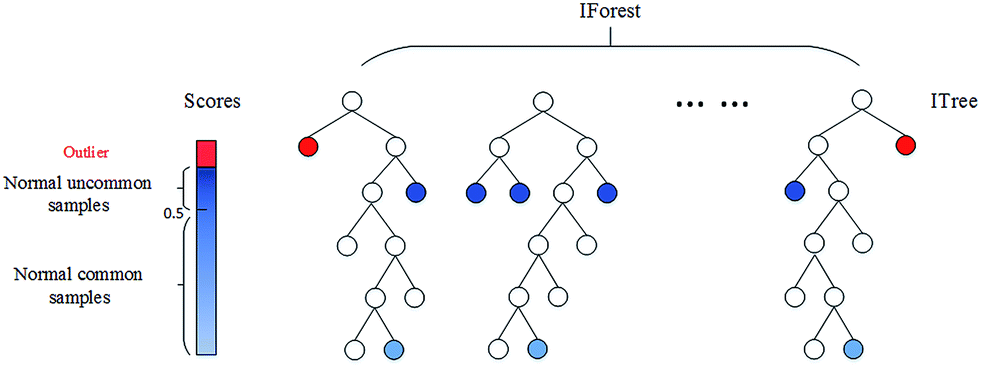
\includegraphics[scale=0.45]{inc/images/iforest-scheme.png}
  \caption{Схема выявления аномалий на основе метода изолирующего леса \cite{Short-outlier-methods-overview}}
  \label{fig:iforest-scheme}
\end{figure}

Основная идея IForest заключается в том, чтобы вычислить оценку аномалии для каждого наблюдения в наборе данных. Для этого строится лес случайных и независимых бинарных изолирующих деревьев (ITree). Также модель использует два входных параметра: размер выборки $\psi$, случайно выбранный из всего набора данных, и $t$ --- количество деревьев в лесу.

\newpage

Построение очередного ITree происходит следующим образом:
\begin{itemize}[leftmargin=0pt,itemindent=4.6em]
    \item инвариант – корневой узел содержит все наблюдения выборки;
    \item IForest случайным образом выбирает подмножество наблюдений $\psi$;
    \item разделение узла $i$: 
        \begin{itemize}[leftmargin=4.6em,itemindent=4.6em]
            \item[$\bullet$] IForest случайным образом выбирает функцию $f_i$  из заданного набора функций;
            \item[$\bullet$] значение разделения $v_i$ также случайным образом выбирается между $\min(f_i)$ и $\max(f_i)$;
            \item[$\bullet$] элементы узла $i$ разбиваются на левую и правую группы (поддеревья) путем сравнения их значений с $v_i$;
        \end{itemize}
    \item процедура разделения рекурсивно продолжается до тех пор, пока все выборочные данные не будут изолированы или дерево не достигнет максимальной глубины, равной $\log_2 \psi$.
\end{itemize}

Так, чтобы построить $t$ изолирующих деревьев леса, необходимо повторить вышеописанные шаги $t$ раз. Построение IForest представляет собой этап обучения в данном методе.

Для каждого наблюдения можно рассчитать показатель выбросов \cite{Isolation-Forest} по формуле (\ref{s_xn_def}):

\begin{equation}\label{s_xn_def}
    s(\overline{x},\ n) = 2^{-\tfrac{\mu(h(x))}{c(n)}},
\end{equation}
где $h(\overline{x})$ --- число шагов до полной изоляции экземпляра $\overline{x}$, \\
$\mu(h(\overline{x}))$ --- среднее значение $h(\overline{x})$, взятое по ансамблю деревьев, \\
$c(n)$ --- значение нормализации, заданное соотношением (\ref{c_n_def}). \\

\begin{equation}\label{c_n_def}
    c(n) = \begin{cases}
         2H(m - 1) - \dfrac{2(m - 1)}{n}, &\ \text{если } m > 2, \\
         1, &\ \text{если } m = 2, \\ 
         0, &\ \text{иначе}, \\ 
    \end{cases}
\end{equation}
где $n$ --- объем данных тестирования, \\
$m$ --- размер набора выборок, \\
$H(i)$ --- число гармоник, которое можно оценить $H(i)=\ln i + \gamma$, где $\gamma \approx 0,577$ --- постоянная Эйлера-Макерони \cite{Eiler-Maskeroni-Const}.

Таким образом, если значение $s(\overline{x}, n)$ близко к $1$, то экземпляр $\overline{x}$ с большой вероятностью является аномалией. Если $s(\overline{x}, n) < \tfrac{1}{2}$, то $\overline{x}$ , скорее всего, относится к нормальной точке выборки.

Данный метод эффективен для обработки больших объемов данных и обладает высокой скоростью обучения, что делает его привлекательным для решения задач обнаружения аномалий в реальном времени. Однако стоит заметить, что в случае локальных выбросов IForest может справляться хуже, чем с глобальными аномалиями.

Более того, в 2023 году в работе \cite{DIF} было представлено новое расширение --- Deep Isolation Forest (DIF). Метод предлагает ряд существенных преимуществ по сравнению со стандартным методом IForest:

\begin{itemize}[leftmargin=0pt,itemindent=4.6em]
    \item[$\bullet$] эффективность в пространствах высокой размерности;
    \item[$\bullet$] избежание алгоритмического смещения (см. рисунок \ref{fig:iforest-and-dif-comparison}): DIF предоставляет более обширный метод изоляции, который может произвольно разделять данные в любом случайном направлении и угле на подпространствах любого размера;
    \item[$\bullet$] возможность обработки сложных и трудноизолируемых аномалий за счёт использования случайных нейронных сетей, не требующих оптимизации.
\end{itemize}

\begin{figure}
  \centering
  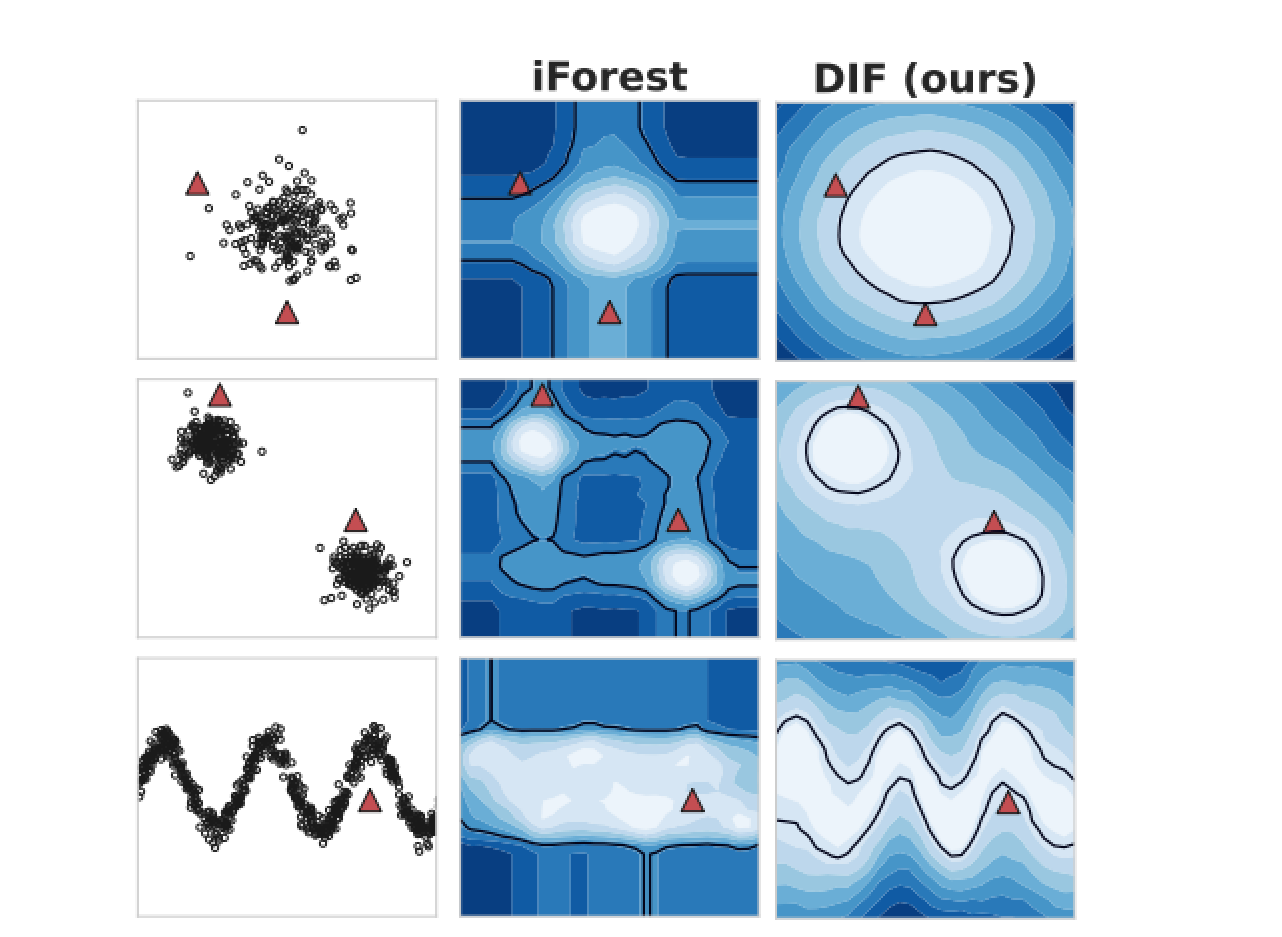
\includegraphics[scale=0.235]{inc/images/iforest-and-dif-comparison.png}
  \caption{Сравнение IForest и DIF: разрешение проблемы алгоритмического смещения при выявлении аномалий \cite{DIF}}
  \label{fig:iforest-and-dif-comparison}
\end{figure}

Таким образом, DIF преодолевает ограничения стандартного IForest, дополняя каноничный метод и предоставляя более гибкое и эффективное средство обнаружения аномалий.

Здесь функция принятия решений $f(\overline{x_i})$ основывается на оценке аномальности $s(\overline{x_i}, n)$, рассчитанной по формуле (\ref{s_xn_def}). Для определения принадлежности экземпляра $\overline{x_i}$ к классу $y_1$ или $y_2$ необходимо установить пороговое значение $s^*$, при превышении которого экземпляр считается аномальным. Таким образом, функция $f(\overline{x_i})$ определяется следующим образом:

\begin{equation}\label{f_iforest_def}
    f(\overline{x_i}) = \begin{cases}
         \ \ 1, &\ \text{если } s(\overline{x_i}, n) \geq s^*, \\
               -1, &\ \text{иначе}.
         \end{cases}
\end{equation}

Выбор порогового значения $s^*$ напрямую влияет на $\alpha$ и $\beta$. Для достижения оптимального баланса между $\alpha$ и $\beta$ необходимо производить калибровку $s^*$ с использованием кросс-валидации.

    \subsection{ECOD}

В марте 2022 года в работе \cite{ECOD} был показан простой, но эффективный алгоритм ECOD (Empirical-Cumulative-distribution-based Outlier Detection), который был вдохновлен тем фактом, что аномалии часто являются «редкими событиями», которые появляются на краях распределения. Данный подход имеет ряд важнейших особенностей, которые стоит отметить:

\begin{itemize}[leftmargin=0pt,itemindent=4.6em]
    \item[$\bullet$] простота понимания и интерпретации метода;
    \item[$\bullet$] отсутствие гиперпараметров, что может быть важно в контексте обнаружения аномалий: их часто может быть сложно корректно настроить, поскольку аномальные экземпляры редки и их не всегда просто получить;
    \item[$\bullet$] в данном методе временная сложность линейно зависит от размера входных данных и числа измерений.
\end{itemize}

ECOD использует информацию о распределении данных, чтобы определить, где данные менее вероятны и, следовательно, более вероятны выбросы. В частности, ECOD оценивает \cite{Replace-Outlier-Detection-with-ECOD} эмпирическую кумулятивную функцию распределения ECDF (см. рисунок \ref{fig:ecdf}) для каждой переменной отдельно.

\begin{figure}
  \centering
  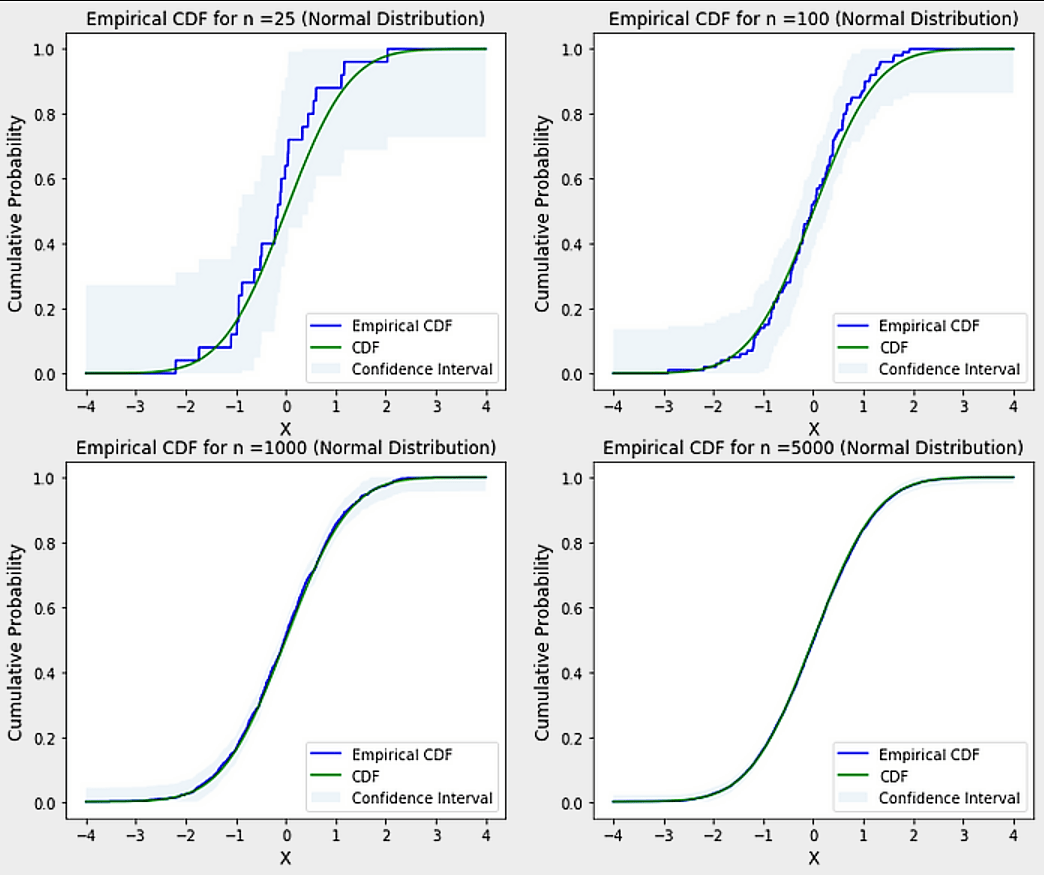
\includegraphics[scale=0.3]{inc/images/ecdf.png}
  \caption{Примеры ECDF для разного объёма выборки нормального распределения \cite{Replace-Outlier-Detection-with-ECOD}}
  \label{fig:ecdf}
\end{figure}

Идеальным вариантом здесь было бы применить объединенный ECDF ко всем переменным; однако это слишком дорого с точки зрения вычислений (скорость сходимости при оценке совместного CDF замедляется по мере увеличения числа переменных). Таким образом, ECOD делает упрощающее предположение о том, что переменные статистически независимы. Но даже с учетом этого предположения ECOD работает довольно хорошо.

Рассмотрим, как работает обучение в данном методе. Пусть на вход поданы данные $X = \{X_i\}_{i=1}^n \in \mathbb{R}^{(n \times d)}$  с $n$ выборками и $d$ признаками. Обозначим $X_i^{(j)}$  значение $j$-го признака для $i$-го экземпляра. Тогда для того, чтобы определить, является ли экземпляр $X_i$  аномалией, необходимо рассчитать 3 вероятностные величины на <<хвостах>> (tails) распределений по формулам (\ref{O_left_def}), (\ref{O_right_def}) и (\ref{O_auto_def}).

\begin{equation}\label{O_left_def}
    O_{left}(X_i)= - \sum\limits_{j=1}^d \log \left[ECDF_{left}^{(j)} (X_i^{(j)} )\right],
\end{equation}
\begin{equation}\label{O_right_def}
    O_{right}(X_i)= - \sum\limits_{j=1}^d \log \left[ECDF_{right}^{(j)} (X_i^{(j)} )\right],
\end{equation}
\begin{equation}\label{O_auto_def}
    O_{auto}(X_i)= \begin{cases}
         - \sum\limits_{j=1}^d \log \left[ECDF_{left}^{(j)} (X_i^{(j)} )\right], &\ \text{если } \gamma_j < 0, \\
         - \sum\limits_{j=1}^d \log \left[ECDF_{right}^{(j)} (X_i^{(j)} )\right], &\ \text{иначе}, \\ 
    \end{cases}
\end{equation}
где $\gamma_j$  – коэффициент асимметрии (skewness) выборки для $j$-го распределения признака (для одной переменной нахождение в левом хвосте распределения вероятностей может быть более аномальным, чем для другой), который, в свою очередь, определяется соотношением (\ref{skewness_coff_def}).
\begin{equation}\label{skewness_coff_def}
    \gamma_j  =  \dfrac{\dfrac{1}{n} \sum\limits_{i = 1}^n \left(X_i^{(j)} - \overline{X^{(j)}}\right)^3}
                       {\left[\dfrac{1}{n-1} \sum\limits_{i = 1}^n \left(X_i^{(j)} - \overline{X^{(j)}}\right)^2 \right]^{^3/_2}}.
\end{equation}

Одно из преимуществ использования отрицательных логарифмов вероятностей заключается в том, что более низкая вероятность преобразуется в более высокое отрицательное логарифмическое значение. Таким образом, редкие элементы с низкой вероятностью получают более высокие оценки аномалий. Тогда результирующую оценку аномальности экземпляра $X_i$ определяется соотношением (\ref{O_def}).

\begin{equation}\label{O_def}
    O(X_i) = \max{ \left\{ O_{left}(X_i),\ O_{right}(X_i),\ O_{auto}(X_i) \right\} } 
\end{equation}


На рисунке \ref{fig:ecod-demo} показано, как комплексный подход к оценке и корректировка асимметрии на основе $\gamma_j$  даёт возможность значительно улучшить результаты в выявлении аномалий в данных. Предложенный метод является эффективным, быстрым и масштабируемым алгоритмом обнаружения аномалий в данных.

\begin{figure}
  \centering
  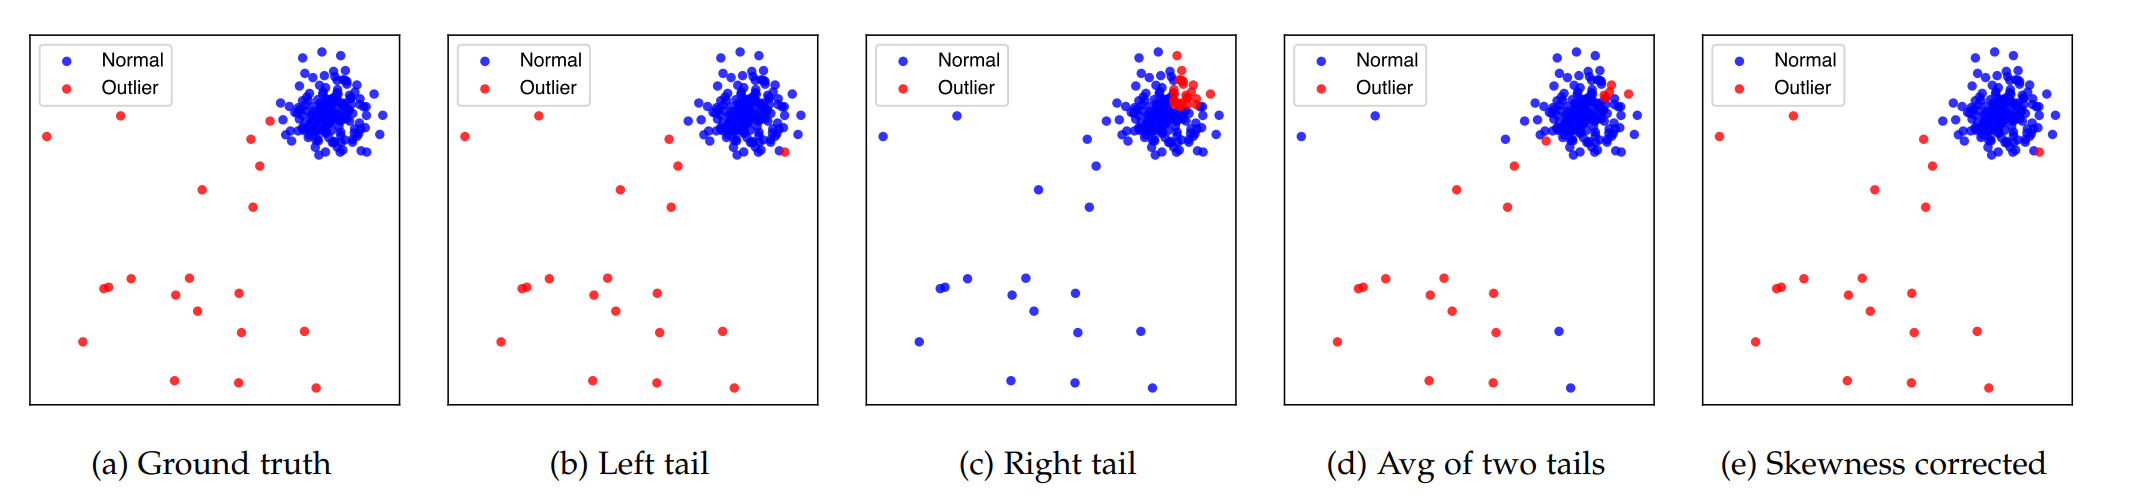
\includegraphics[scale=0.22]{inc/images/ecod-demo.png}
  \caption{Демонстрация влияния «хвостовых вероятностей» и корректировки асимметрии на выявление аномалий \cite{ECOD}}
  \label{fig:ecod-demo}
\end{figure} 

Функция принятия решений (\ref{f_ecod_def}) формализуется через задание порогового значения $\tau \in \mathbb{R}^+$, определяемого на основе концепции  уровня контаминации (англ. \textit{contamination rate}) $\rho \in [0,1]$, который задаёт ожидаемую долю аномалий в данных. Для этого:
\begin{enumerate}[leftmargin=0pt,itemindent=4.6em]
    \item[1.] все экземпляры ранжируются по убыванию оценок $O(X_i)$;
    \item[2.] $\tau$ устанавливается в (\ref{tau_ecod_def}) как $(1-\rho)$-квантиль полученного распределения оценок:
\end{enumerate}

\begin{equation}\label{tau_ecod_def}
    \tau = Q_{1-\rho}\left( \{ O(\overline{x_j}) \ |\ \forall \overline{x_j} \in X \} \right),
\end{equation}
где $Q_{1-\rho}$ --- оператор квантиля уровня $(1-\rho)$. 

\newpage
Сама функция:

\begin{equation}\label{f_ecod_def}
    f(\overline{x_i}) = \begin{cases}
         \ \ 1, &\ \text{если } O(\overline{x_i}) \geq \tau, \\
         -1, &\ \text{иначе}. 
    \end{cases}
\end{equation}

Данный подход соответствует описанию метода ECOD в оригинальной работе \cite{ECOD}, где:
\begin{itemize}[leftmargin=0pt,itemindent=4.6em]
    \item[$\bullet$] оценки $O(X_i)$ вычисляются независимо для каждого измерения через эмпирические хвостовые вероятности (уравнения \ref{O_left_def}--\ref{O_auto_def});
    \item[$\bullet$] порог $\tau$ адаптируется к данным через квантильный критерий, что устраняет необходимость явных предположений о распределении нормальных экземпляров;
    \item[$\bullet$] уровень значимости $\alpha$ косвенно контролируется через параметр $\rho$, который может быть настроен в соответствии с требованиями задачи.
\end{itemize}

Минимизация $\beta$ достигается за счёт следующих свойств ECOD:
\begin{itemize}[leftmargin=0pt,itemindent=4.6em]
    \item[$\bullet$] использование логарифмических преобразований хвостовых вероятностей усиливает контраст между типичными и редкими событиями;
    \item[$\bullet$] адаптивный выбор хвоста через коэффициент асимметрии $\gamma_j$ (формула \ref{skewness_coff_def}) улучшает чувствительность к мультимодальным распределениям;
    \item[$\bullet$] агрегация через $\max$-оператор фокусируется на наиболее аномальных измерениях.
\end{itemize}






    \subsection{Автокодировщик для обнаружения аномалий}

Также для решения задачи обнаружения аномалий было рассмотрено применение автокодировщиков (или автоэнкодеров, англ. autoencoder). Представляет собой архитектурный класс искусственных нейронных сетей, которая использует метод обучения без учителя с применением алгоритма обратного распространения ошибки.

В применении автокодировщиков для обнаружения аномалий используется их основное свойство --- необходимость фиксировать в скрытом латентном слое, полученном с помощью кодера (англ. encoder), наиболее важной информации о входном сигнале для его последующего восстановления декодером (англ. decoder). Благодаря этому свойству автокодировщик способен восстанавливать знакомый ему сигнал, считающийся нормальным, и не может восстановить аномальный сигнал, содержащий неизвестные паттерны. Это свойство и заложено в основе применения автокодировщиков для обнаружения аномалий.

Рассмотрим нейронную сеть автокодировщика с единственным скрытым слоем. Она будет иметь кодер и декодер, заданные соотношениями (\ref{h_def}) и (\ref{z_def}), соответственно.

\begin{equation}\label{h_def}
    \overline{h} = \sigma(W_{xh} \overline{x} + \overline{b_{xh}}),
\end{equation}

\begin{equation}\label{z_def}
    \overline{z} = \sigma(W_{hx}\overline{h} + \overline{b_{hx}}),
\end{equation}
где $W$ и $\overline{b}$ --- вес и смещение (англ. bias) нейронной сети, \\
$\sigma$ --- функция нелинейного преобразования.

Кодер в уравнении (\ref{h_def}) отображает входной вектор $\overline{x}$ в скрытое представление $\overline{h}$ с помощью нелинейного преобразования. Декодер в (\ref{z_def}) отображает скрытое представление $\overline{h}$ обратно в $\overline{z}$ исходного пространство с помощью того же преобразования, что и кодер. Разница между исходным входным и восстановленным векторами называется ошибкой восстановления, как показано в формуле (\ref{e_def}).

\begin{equation}\label{e_def}
    e =  \lVert \overline{x} - \overline{z} \rVert.
\end{equation}

Автокодировщик обучатся минимизировать $e$. Алгоритм обучения нативного автоэнкодера показан в алгоритме~\ref{alg:AE_train}, где $f_{\phi}$ и $g_{\theta}$ - многослойные нейронные сети для автокодировщика.

\begin{algorithm}[htp!]
    \caption{Стандартное обучение автокодировщика} \label{alg:AE_train}
    \SetAlgoLined %% Это соединяет линиями логические части
    \KwData{Набор данных $\overline{x_1}, ..., \overline{x_n},\ n < k$}
    \KwResult{ обученные $f_{\phi}$ и $g_{\theta}$ }
    
    Инициализировать параметры $\phi$ и $\theta$ \\
    \While{ не достигнута сходимость $\phi$ и $\theta$}{
        // Вычисление суммарной ошибки восстановления. \\
        $E = \sum\limits_{i = 1}^n\lVert \overline{x_i} - g_{\theta}(f_{\phi}(\overline{x_i})) \rVert$ \\
        $\phi,\ \theta \leftarrow$ Обновление параметров с помощью градиента $E$ (например, стохастический градиентный спуск) \\
    }
    \Return{$f_{\phi}$, $g_{\theta}$}
\end{algorithm}

Обнаружение аномалий на основе автокодировщика --- это метод обнаружения аномалий на основе отклонений, использующий обучение с частичным привлечением учителя (англ. semi-supervised learning). Он использует ошибку восстановления в качестве оценки аномалии. Точки данных с высокой значением $e$ считаются аномалиями. 

Для обучения автоэнкодера используются только данные с нормальными экземплярами. После обучения автоэнкодер будет очень хорошо восстанавливать нормальные данные, но не сможет сделать этого с аномальными данными, с которыми автоэнкодер не сталкивался. Алгоритм \ref{alg:AE_detector} демонстрирует обнаружение аномалий с использованием ошибок восстановления автокодировщиков.

\newpage

\begin{algorithm}[htp!]
    \caption{Обнаружение аномалий на основе автокодировщика} \label{alg:AE_detector}
    \SetAlgoLined %% Это соединяет линиями логические части
    \KwData{ \\
        Набор \textbf{нормальных} данных $X' \subset X,\ |X'| = n < k$, \\
        Набор неразмеченных данных (потенциально аномальных)  $\overline{x'_1}, ..., \overline{x'_l} $, \\
        Метки классов $Y = \{y_1,\ y_2\}$, где $y_1$ --- <<аномальный>>, \\
        $\phantom \qquad\qquad\qquad\qquad\qquad\qquad\qquad\quad\ y_2$ --- <<нормальный>>, \\
        Порог ошибки $\epsilon$.
    }
    \KwResult{ значение ошибки восстановления $e =  \lVert \overline{x} - \overline{z} \rVert$ }
    
    $\phi,\ \theta \leftarrow$ обучить, используя набор <<нормальных>> данных $X'$ \\
    \For {$i := \overline{1,\ l}$} {
        $error(i) = \lVert \overline{x_i} - g_{\theta}(f_{\phi}(\overline{x_i})) \rVert$ \\
        \eIf{$error(i) > \epsilon$}{
		$\overline{x_i}$ помечается, как принадлежащий классу $y_1$
	}{ 
		$\overline{x_i}$ помечается, как принадлежащий классу $y_2$
	}
    }
\end{algorithm}

Рассмотрим архитектуру нейронной сети автокодировщика, представленной на рисунке \ref{fig:autoencoder-scheme}, которая может быть применена для обнаружения аномалий сетевого трафика.

\begin{figure}
  \centering
  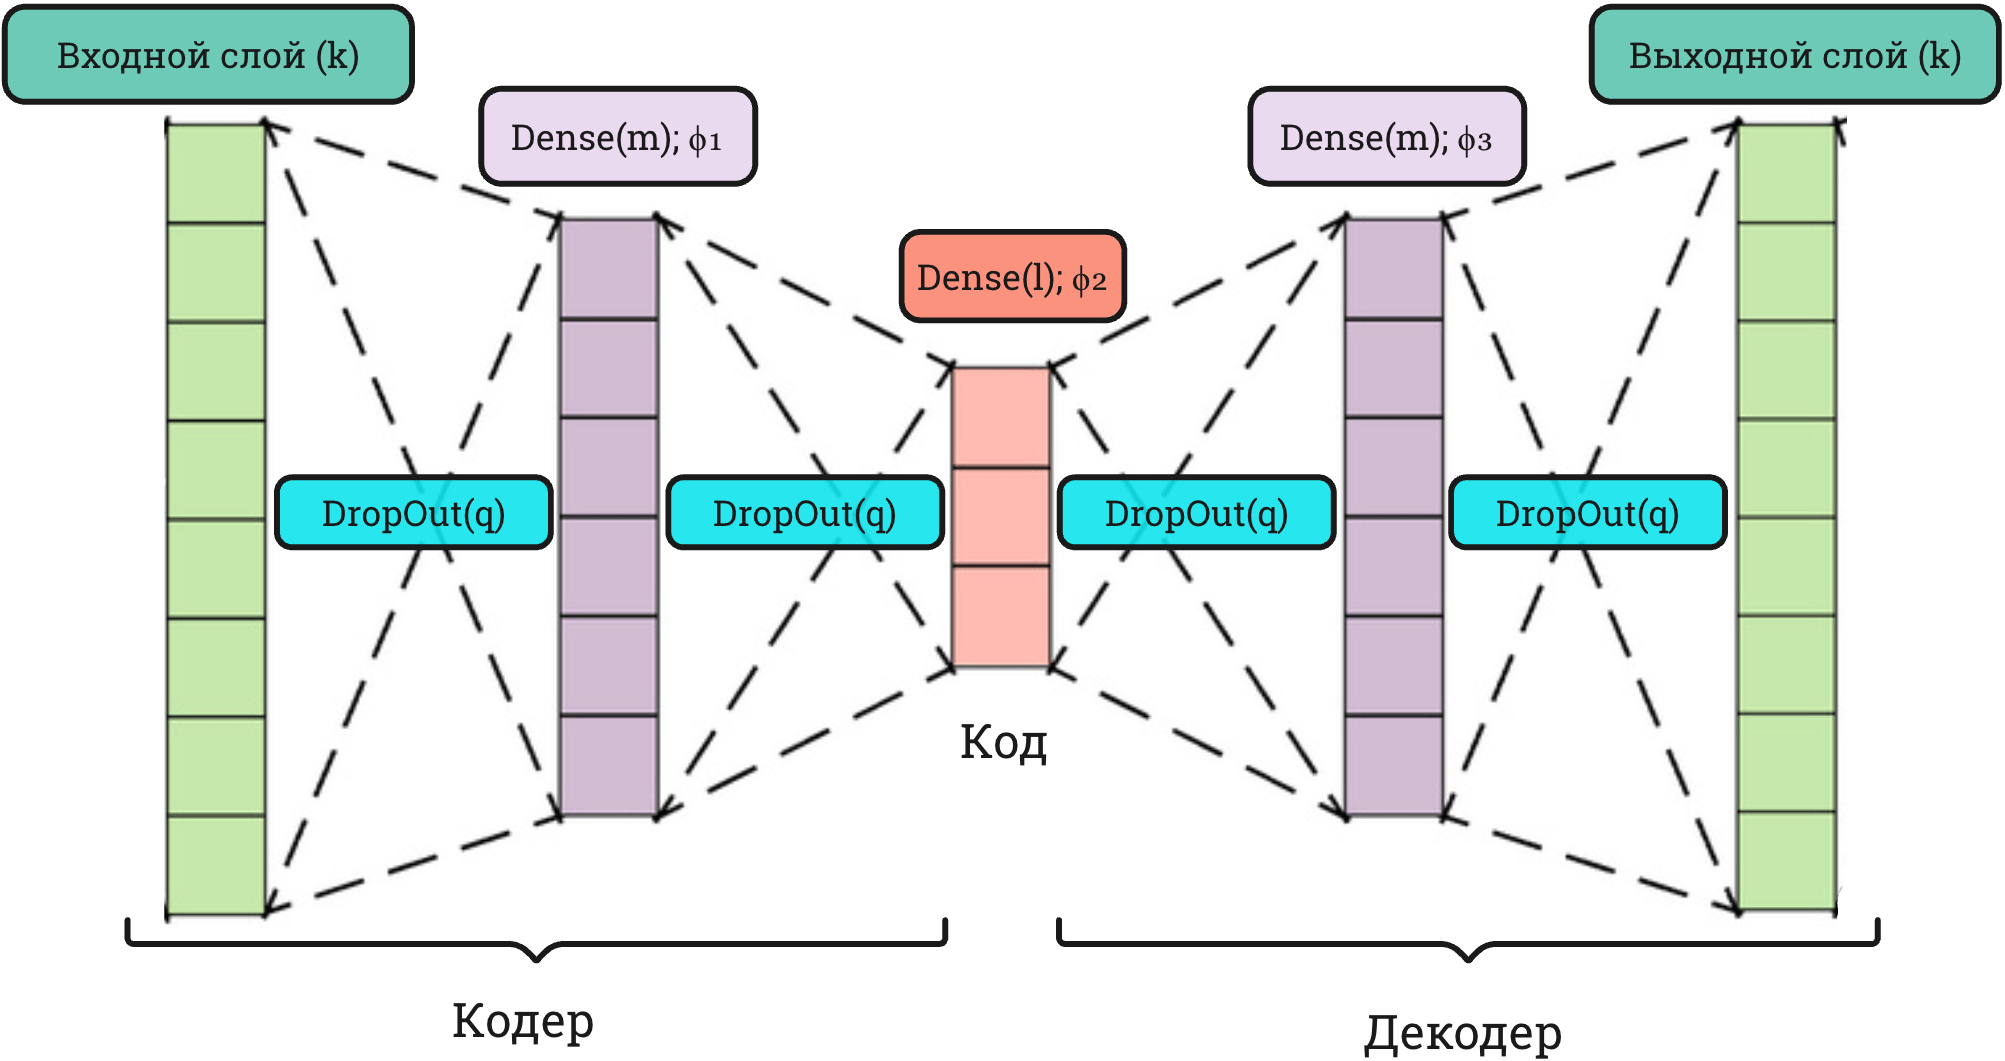
\includegraphics[scale=0.23]{inc/images/autoencoder-scheme.png}
  \caption{Архитектура искусственной нейронной сети автокодировщика для обнаружения аномалий в сетевом трафике}
  \label{fig:autoencoder-scheme}
\end{figure}

Входной и выходной слои имеют количество нейронов по числу признаков, извлечённых в элементы $X$ из множества $T$ по формуле (\ref{X_def}). Скрытые слои энкодера и декодера содержат $m$ и $l$ нейронов соответственно.

Каждый слой использует функции активации $\phi_1$, $\phi_2$ и $\phi_3$ для введения нелинейности в модель. Примером хорошо зарекомендовавшей себя функции активации может послужить линейный выпрямитель (или полулинейный элемент, англ. \textit{Rectified linear unit}, ReLU), представленный формулой (\ref{relu_def}). Она монотонна, что гарантированно делает выпуклой поверхность ошибок, ассоциированную с одноуровневой моделью. Также ReLU --- гладкая, то есть имеет монотонную производную, что в некоторых случаях обеспечивает более высокую степень общности.

\begin{equation}\label{relu_def}
    \phi(x) = 
    \begin{cases}
        0, &\ \text{если } x < 0, \\
        x, &\ \text{если } x \ge 0. \\ 
    \end{cases}
\end{equation}

Также в автокодировщике применяется метод регуляризации \textit{Dropout} с параметром $q \in (0;\ 1)$, что помогает предотвратить переобучение, случайным образом отключая $q \cdot 100\%$ нейронов во время обучения. 

Обучение автокодировщика может осуществляться с использованием функции потерь $MSE$ (англ. \textit{Mean Squared Error} --- среднеквадратичная ошибка), которая измеряет разницу между входными данными и восстановленными данными. Далее результаты восстановления декодера сравниваются с входным слоем для оценки аномальности экземпляра данных. Среднеквадратичная ошибка определяется соотношением $MSE = \sigma^2$, где $\sigma$ --- стандартное отклонение, ранее определённое в формуле (\ref{standard_deviation}).


    \section{Обоснование решения математической постановки задачи}

В конечном итоге, обнаружение аномалий в сетевом трафике решено построить на базе автокодировщиков. Этот выбор обусловлен успешностью применения данного класса моделей для решения поставленной задачи и оптимизации параметра $\beta$ при установленном значении порога $\alpha$, что показано в результатах работ \cite{Gurina2019AnomalyBasedMF}, \cite{Applied-Autoencoder-One}, \cite{Applied-Autoencoder-Two}. Также это подтвердили численные эксперименты, проводимые в рамках прошедших НИРС.

Автокодировщики обладают способностью эффективно обрабатывать высокоразмерные данные, что является важным аспектом при анализе сетевого трафика, где количество признаков может быть значительным. Они способны выявлять сложные паттерны в данных благодаря своей архитектуре. Это позволяет им адаптироваться к различным типам данных и выявлять аномалии, которые могут быть неочевидны для других методов.

Также данный метод позволяет осуществить тонкую настройку за счёт установки параметров скрытых полносвязных слоёв нейросети автоэнкодера, выбора оптимальных функций активации, применения метода регуляризации \textit{Dropout} с подбором процента исключения случайных нейронов, что повышает итоговое качество предсказаний модели, а также подбор функции потерь и оптимизатора нейронной сети. 

    \conclusion

В данной работе была сформулирована математическая постановка задачи обнаружения аномалий в сетевом трафике на основе машинного обучения. Были предложены пути решения поставленной задачи, выбран и описан оптимальный алгоритм для её решения. В результате решение настоящей задачи будет построено на базе нейронной сети автокодировщика, хорошо зарекомендовавшего себя по результатам опубликованных работ и численных экспериментов, проводимых ранее в рамках НИРС.

Специфика предметной области и сам тип аномалий представляет особые вызовы для существующих методов их обнаружения. На основе анализа проблемы, технических и функциональных особенностей, реализуемых в информационной системе, делается выбор в пользу тех или иных методов решения поставленной задачи. Действительно, вредоносная активность имеет тенденцию выглядеть нерегулярно по сравнению с повседневными операциями, что позволяет свести данную проблему к задаче поиска аномалий в данных сетевого трафика, поступающего как из сети Интернет, так и циркулирующего в контуре организации.

Системы, основанные на заранее настроенных сигнатурах и правилах, зачастую будут <<слепы>> к атакам нулевого дня, в то время как anomaly-based-решения способны выявить подозрительную активность на основе алгоритмов машинного обучения, что будет отражено в выпускной квалификационной работе специалиста.


    \printbibliography[env=nirs-bibliography]
\end{document}
